%% Background
\chapter{Methodology}
\label{chap:methodology}

\section{Data Collection}

We downloaded 6,018 TrueType (.ttf) and OpenType (.otf) font files from Google Fonts using the macOS FontBase software. We then used the FontForge library Python scripting to create a database of images of each common character\footnote{Capital letters (A-Z), lowercase letters (a-z), numbers (0-9), punctuation, and basic symbols} represented in each typeface, totalling 556,123 glyph images. The script also created a .csv file containing the locations of each character-font combination image in our database for use later in model training.

\section{Models}

We employed several models in attempting to create a useful latent style encoding of  typefaces in our dataset. This section details these model architectures and our approach to implementing them. All models were trained in PyTorch 2.4.1 running on a Bizon G7000 G2 GPU server with 2x 32-Core 2.00 GHz Intel Xeon Gold 6338 CPUs and 4x NVIDIA RTX A6000 48 GB GPUs.

\subsection{Autoencoder}

Our first attempt at building a model to encode font style was a simple autoencoder. An autoencoder, first introduced in \cite{rumelhart1986}, is a neural network trained to compress and reconstruct input data. A simple diagram of the autoencoder model is shown in Figure \ref{fig:autoencoder-model}. The autoencoder model consists of two parts: an encoder, which compresses the data to a smaller vector representation, and a decoder which expands it back out to the original size. The model trains on a loss function which computed the MSE across each pixel value between the input and output images.

% from Bank et al. "Autoencoders"
\begin{figure}[h]
    \centering
    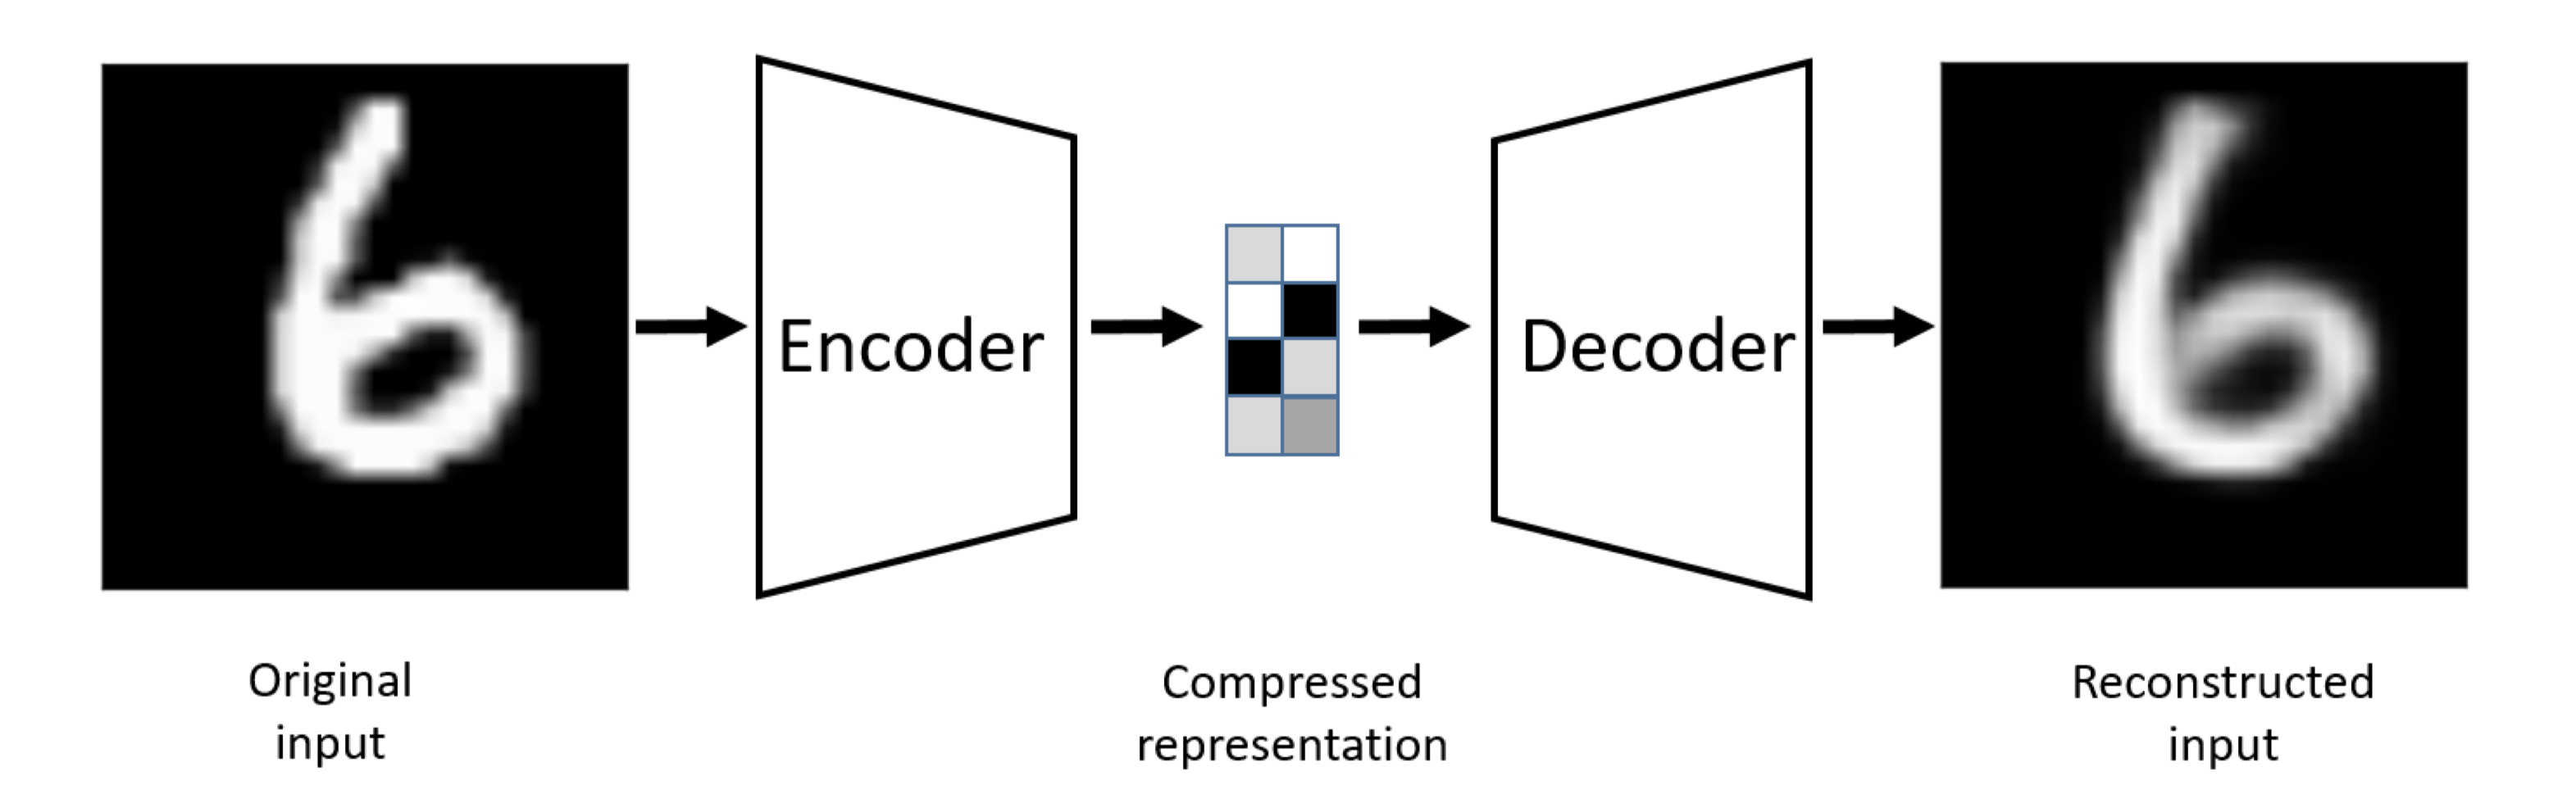
\includegraphics[width=\textwidth]{images/autoencoder-model.png}
    \caption{A basic autoencoder model applied on MNIST data, as shown in \cite{rumelhart1986}.}
    \label{fig:autoencoder-model}
\end{figure}

We implemented an autoencoder model to encode all characters in our database, using a combination of alternating linear layers and ReLU activation functions for both our encoder and decoder. As we experimented with multiple image sizes for our model ($28\times28$, $56\times56$, $112\times112$), we varied the shape of our architecture accordingly; in general, however, each layer of the decoder reduced the input size by a factor of $\frac{1}{2}$ and each layer of the encoder expanded the vector size by approximately a factor of 2. We also experimented with different sizes for the size of the internal compressed representation, however we settled on a hidden layer size of $H=10$.

\subsection{Style Transfer}

In an attempt to more specifically encode the style of fonts as separate from their content, we modified the autoencoder architecture to train a model to recreate \textit{other} characters in a given font, based on a font glyph and two input character embeddings. For example, given an input image of a ``C'' character in given font, our model might train to recreate the known ``X'' character in that same font. (In reality, our model would train on recreating \textit{every} character given \textit{every other} character in each font in our dataset).

In order to implement this model, we encountered an early difficulty: not every font in our dataset contained every character we wanted to train on. To remedy this, we limited our sample size to only include fonts which contained all lowercase (a–z) and uppercase (A–Z) English characters, and trained our style transfer model only on these characters. This eliminated 129 fonts, leaving us with alphabetic fonts. We proceeded building our model around these fonts and character sets.

There were two main differences between our style transfer model and the original autoencoder model from which we adapted it. First of all, we had to significantly modify the data loading process: although we were working with a smaller subset of character options (ignoring numbers, punctuation, and special characters), our dataset was actually much \textit{larger} given that we had to consider every combination of characters in a font, rather than every individual character in a font. It was necessary to modify our dataloader to provide, for each entry in the dataset, the input truth, the output truth (which the model was trying to reconstruct), and the input/output characters. The other change we implemented in this model was actually feeding these new data into the model. We created two tensor embeddings of the input/output characters; the input embedding was concatenated to the input image before it was fed through the encoder, and the output embedding was concatenated between the encoder and decoder steps. Finally, we computed the MSE loss not against the input image but against the ground truth goal image provided by the dataloader.

Figure \ref{fig:styletransfer-example} shows our style transfer model part-way through training. The model receives the input \textbf{B} glyph and the input/output character embeddings, and it attempts to create the \textbf{h} glyph in the same typeface.

% my own figure
\begin{figure}[h]
    \centering
    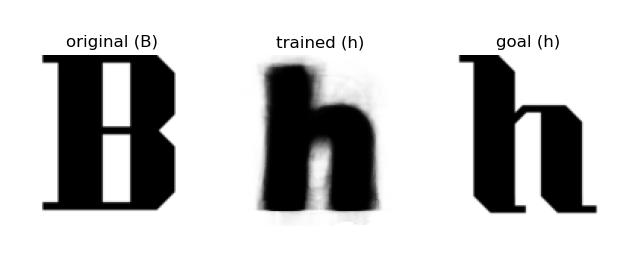
\includegraphics[width=\textwidth]{images/styletransfer-example.png}
    \caption{An example of our style transfer model part-way through training.}
    \label{fig:styletransfer-example}
\end{figure}

By giving the model explicit vector representation of the input/output characters, we hypothesized that the model would more effectively isolate the style of the glyphs as separate from their content, giving us better internal model embeddings to leverage for font style selection.